% Report for YAMS, project in CWRU EECS 314 Spring 2015
%
% Members:
%    Stephen Brennan (smb196)
%    Katherine Cass (krc53)
%    Jeffrey Copeland (jpc86)
%    Andrew Mason (ajm188)
%    Thomas Murphy (trm70)
%    Aaron Neyer (agn31)

\documentclass[journal,10pt]{IEEEtran}
% Will correctly load from ./
% Explicit use of 10pt by report requirements

% *** GRAPHICS RELATED PACKAGES ***
%
\ifCLASSINFOpdf
 \usepackage[pdftex]{graphicx}
\else
 \usepackage[dvips]{graphicx}
\fi

% declare the path(s) where your graphic files are
 \graphicspath{{screenshots/}}
% declare graphics file extensions
\DeclareGraphicsExtensions{.pdf,.jpeg,.png}

% *** MATH PACKAGES ***
%
\usepackage[cmex10]{amsmath}

% *** PDF, URL AND HYPERLINK PACKAGES ***
%
\usepackage{url}
% url.sty was written by Donald Arseneau. It provides better support for
% handling and breaking URLs.
% Basically, \url{my_url_here}.

% Correctly create hyperlinks with URLs
\usepackage{hyperref}

% Allow nicer float options
\usepackage{float}

% correct bad hyphenation here
\hyphenation{op-tical net-works semi-conduc-tor}


\begin{document}
%
% paper title
% Titles are generally capitalized except for words such as a, an, and, as,
% at, but, by, for, in, nor, of, on, or, the, to and up, which are usually
% not capitalized unless they are the first or last word of the title.
% Linebreaks \\ can be used within to get better formatting as desired.
% Do not put math or special symbols in the title.
\title{YAMS: Awesome MIPS Server}
% Title is still up for consideration

%
%
% author names and IEEE memberships
% note positions of commas and nonbreaking spaces ( ~ ) LaTeX will not break
% a structure at a ~ so this keeps an author's name from being broken across
% two lines.
% use \thanks{} to gain access to the first footnote area
% a separate \thanks must be used for each paragraph as LaTeX2e's \thanks
% was not built to handle multiple paragraphs
%

\author{
Stephen~Brennan,
Katherine~Cass,
Jeffrey~Copeland,
Andrew~Mason,
Thomas~Murphy,
Aaron~Neyer% stop_space
\thanks{All authors are with the Department of Electrical Engineering and Computer Science, Case Western Reserve University, Cleveland, OH, 44106 USA}% stop_space
\thanks{Final Report submitted May 1, 2015, typographical revisions \today}
} % Close the author environment

% note the % following the last \IEEEmembership and also \thanks -
% these prevent an unwanted space from occurring between the last author name
% and the end of the author line. i.e., if you had this:
%
% \author{....lastname \thanks{...} \thanks{...} }
%                     ^------------^------------^----Do not want these spaces!
%
% a space would be appended to the last name and could cause every name on that
% line to be shifted left slightly. This is one of those "LaTeX things". For
% instance, "\textbf{A} \textbf{B}" will typeset as "A B" not "AB". To get
% "AB" then you have to do: "\textbf{A}\textbf{B}"
% \thanks is no different in this regard, so shield the last } of each \thanks
% that ends a line with a % and do not let a space in before the next \thanks.
% Spaces after \IEEEmembership other than the last one are OK (and needed) as
% you are supposed to have spaces between the names. For what it is worth,
% this is a minor point as most people would not even notice if the said evil
% space somehow managed to creep in.



% The paper headers
\markboth{CWRU EECS 314 Spring 2015 Final Project}%
{}
% The only time the second header will appear is for the odd numbered pages
% after the title page when using the twoside option.



% make the title area
\maketitle

% As a general rule, do not put math, special symbols or citations
% in the abstract or keywords.
\begin{abstract}
We set out to build a simple web server in MIPS. Mission Accomplished.
\end{abstract}

% Note that keywords are not normally used for peerreview papers.
\begin{IEEEkeywords}
MIPS, computer architecture, HTTP, server, MARS, ISA simulation.
\end{IEEEkeywords}

% Begin body of the report

\section{Problem Statement}
% The very first letter is a 2 line initial drop letter followed
% by the rest of the first word in caps.
%
% form to use if the first word consists of a single letter:
% \IEEEPARstart{A}{demo} file is ....
%
% Here we have the typical use of a "T" for an initial drop letter
% and "HIS" in caps to complete the first word.
\IEEEPARstart{T}{he} goal of this project was to write a static HTTP server in
MIPS and MARS. The server would be able to serve a website, which is contained
in the \texttt{html/} directory on port 19001, which can be viewed in a browser.
Sockets were used for networking and were made available to MIPS by extending
MARS syscalls.


\section{Major Challenges}

One major challenge in YAMS was implementing socket syscalls.
MARS was chosen early on because it allowed for custom syscalls; however,
limited documentation is available. This required us to learn about MARS
through lots of trial-and-error. Additionally, if one stops MARS while
waiting on a socket syscall, the system enters weird error states, forcing
us to either 1) double-reassemble-run the program, or 2) restart all of MARS.
This made debugging much slower than a normal MIPS program.

The larger challenge in implementing YAMS was parsing HTTP requests. RFC
2616\cite{Leach}, our HTTP (Hypertext Transfer Protocol) reference for this
project, is 175 pages long, While it is possible to implement a full HTTP stack
in assembly, it is difficult to do in a month or two. Thus, we focused on what
was required to get web pages to display in a browser: GET, POST, Expect, and
only identity encoding or Content-Length. Additionally, because the request
parser had to interact with the socket depending on various headers (e.g.
Transfer-Encoding, Content-Length, and Expect) Testing and debugging revolved
around trial-and-error requests with the Unix program \texttt{curl} or a browser.

\section{System Components}

Upon submission of the report, the entirety of the implementation will be available at \cite{Brennan}. The breakdown of the system components is as follows.

\subsection{String Operations}

In order to parse HTTP requests, we needed to implement a fair amount of the C
standard string library.  In \texttt{mips/string.asm}, we implemented
\texttt{strlen}, \texttt{strncpy}, \texttt{memcpy}, \texttt{strcmp},
\texttt{strncmp}, \texttt{atoi}, \texttt{htoi}, \texttt{strcat},
\texttt{strncat}, as well as two functions for identifying the index of
characters and substrings, \texttt{str\_index\_of} and
\texttt{substr\_index\_of} respectively.  To verify their correctness, we wrote
tests in \texttt{mips/test\_string.asm}.  They can be run in MARS by loading
that file as the main file, instead of \texttt{mips/main.asm}.

\subsection{HTTP Request Handling}

As mentioned in Major Challenges, our focus with request parsing was on serving
a page that a browser could render. Therefore, we support a subset of HTTP
request statuses (e.g. GET, POST) look for a few headers (e.g. Content-Length,
Expect) and read or write accordingly. The logic for request parsing is in
\texttt{http-requests.asm}, and is reached through the \texttt{get\_request}
method from main, returning an internal HTTP request type, and, as applicable,
request URI, request body, request body length, and content type. The main
method takes this data, and hands it off to the file loader and response builder.

The request parser was determined to be working through trial-and-error, seeing
if debug prints contained the right information and if the browser loaded the
page properly. The mixture of MIPS assembly and MARS syscall extensions
precluded the use of unit tests to verify the correctness of the parser's
behavior.

\subsection{File Access}

Accessing files was already possible through MARS syscalls, saving us the
trouble of adding this feature to the simulator. These calls were wrapped in
function-like macros for ease of use.

Additionally, the HTTP handling receives URIs (uniform resource identifiers),
not system paths. These strings needed processing to produce a valid file path
that could be consumed by the MARS syscall. Our processing, implemented in
\texttt{mips/file.asm}, is composed of substring-blacklisting to prevent the
\texttt{../} directory from being used to escape into uncontrolled resources and
string operations to modify the URI into a useful file path. The file path is
created using the default \texttt{html/} directory (where our web resources are
stored) and URIs with a trailing \texttt{/} have the file name
\texttt{index.html} appended.The processing operation has tests implemented in
\texttt{mips/test\_file.asm}.

\subsection{Turing Tape Language Interpreter}

As an additional ``stretch'' feature, we implemented an interpreter for the
esoteric programming language Brainfuck\cite{Mpreu/preller}.  This simple
language simulates a Turing machine's operations and has only 8 commands (each
of which is a single character).  The interpreter is implemented in
\texttt{mips/brainfuck.asm}, and tested in \texttt{mips/test\_brainfuck.asm}.
When the server is running, code can be loaded into the interpreter by sending a
POST request to the URL \texttt{/load}.  The code can then be run by sending
input in a POST request to the URL \texttt{/run}, which will return the program
output in its response.  As a more simple interface, the URL
\texttt{/brainfuck.html} contains a simple page that uses JavaScript to send
code and input, and receive output, from the interpreter.

\section{Component Integration}

In order to integrate these several different components, we had to define and
follow a strict ``calling convention.''  We decided that all functions would be
called using the \texttt{AL} instruction.  Only the \texttt{\$s0-\$s7} saved
registers, and global pointers, were to be preserved across function calls.
Arguments were passed (and not necessarily preserved) in the \texttt{\$a0-\$a3}
registers, and return values were placed in the \texttt{\$v0-\$v1} registers.
Any additional arguments or return values were to be placed on the stack.
Additionally, it is the caller's responsibility to push any registers which it
wants preserved to the stack.  To facilitate these rules, we defined macros in
\texttt{mips/util-macros.asm} for pushing and popping from the stack, to make
that operation semantically clear in our code.

\section{User Interface}

We have implemented an HTTP server, so there isn't really a ``user interface''
per se. To compile Mars with our implemented syscalls, run make from the project
root. Then run \texttt{java -jar Mars4\_5-SockMod.jar}. You are now running the
modified version of Mars. You can then load in the \texttt{mips/main.asm} file.
Assemble and run that, and you will have a server listening on port 19001. Now,
you can point your browser to any file in the \texttt{html/} directory (but
leave off the \texttt{html/} part of the path - that directory is considered to
be root by the server). Alternatively, you can use the Unix tool \texttt{curl}.

\section{Documentation of Runs}

\subsection{Static Page Content}

The static page in Fig.~\ref{fig:static_document} is hosted as the
\texttt{/index.html} document of the server. This is the document the user would
expect to load into their browser upon access to the root page of the server.
This demonstrates the ability to serve multiple resources for a page: images,
fonts, and the HTML.

\subsection{Dynamic JavaScript Content}

The dynamic page in Fig.~\ref{fig:dynamic_document} is the presentation given to
the class on April 23, 2015. This document uses HTML, JavaScript, and images.
All resources are loaded from YAMS and not from external internet hosts.

\subsection{Interactive AJAX Content}

The final dynamic-content page shown in Fig.~\ref{fig:interactive_ajax} is the
front end interface for the YAMS server's Brainfuck\cite{Mpreu/preller}
interpreter. The page interacts with the interface through POST requests and
updates the text field on the page when it receives the result of running the
user-supplied Brainfuck code and input.

\section{Group Member Contributions}

\begin{LaTeXitemize} \itemsep0pt \parskip0pt
  \item Stephen Brennan
  \begin{enumerate}
    \item String functions
    \item Brainfuck interpreter
  \end{enumerate}

  \item Katherine Cass
  \begin{enumerate}
    \item Static site
    \item Report content
  \end{enumerate}

  \item Jeffrey Copeland
  \begin{enumerate}
    \item Socket Syscalls
    \item HTTP Request Handling
  \end{enumerate}

  \item Andrew Mason
  \begin{enumerate}
    \item HTTP Response Building
    \item Project Presentation
  \end{enumerate}

  \item Thomas Murphy
  \begin{enumerate}
    \item File access
    \item Code formatting and style
    \item Report organization and typesetting
  \end{enumerate}

\end{LaTeXitemize}

Aaron Neyer planned to build a website documenting our project, but could not
complete it due to personal circumstances.

% An example of a floating figure using the graphicx package.
% Note that \label must occur AFTER (or within) \caption.
% For figures, \caption should occur after the \includegraphics.
% Note that IEEEtran v1.7 and later has special internal code that
% is designed to preserve the operation of \label within \caption
% even when the captionsoff option is in effect. However, because
% of issues like this, it may be the safest practice to put all your
% \label just after \caption rather than within \caption{}.
%
% Reminder: the "draftcls" or "draftclsnofoot", not "draft", class
% option should be used if it is desired that the figures are to be
% displayed while in draft mode.
%
%\begin{figure}[!t]
%\centering
%\includegraphics[width=2.5in]{myfigure}
% where an .eps filename suffix will be assumed under latex,
% and a .pdf suffix will be assumed for pdflatex; or what has been declared
% via \DeclareGraphicsExtensions.
%\caption{Simulation results for the network.}
%\label{fig_sim}
%\end{figure}

% Note that IEEE typically puts floats only at the top, even when this
% results in a large percentage of a column being occupied by floats.


% An example of a double column floating figure using two subfigures.
% (The subfig.sty package must be loaded for this to work.)
% The subfigure \label commands are set within each subfloat command,
% and the \label for the overall figure must come after \caption.
% \hfil is used as a separator to get equal spacing.
% Watch out that the combined width of all the subfigures on a
% line do not exceed the text width or a line break will occur.
%
%\begin{figure*}[!t]
%\centering
%\subfloat[Case I]{\includegraphics[width=2.5in]{box}%
%\label{fig_first_case}}
%\hfil
%\subfloat[Case II]{\includegraphics[width=2.5in]{box}%
%\label{fig_second_case}}
%\caption{Simulation results for the network.}
%\label{fig_sim}
%\end{figure*}
%
% Note that often IEEE papers with subfigures do not employ subfigure
% captions (using the optional argument to \subfloat[]), but instead will
% reference/describe all of them (a), (b), etc., within the main caption.
% Be aware that for subfig.sty to generate the (a), (b), etc., subfigure
% labels, the optional argument to \subfloat must be present. If a
% subcaption is not desired, just leave its contents blank,
% e.g., \subfloat[].


% An example of a floating table. Note that, for IEEE style tables, the
% \caption command should come BEFORE the table and, given that table
% captions serve much like titles, are usually capitalized except for words
% such as a, an, and, as, at, but, by, for, in, nor, of, on, or, the, to
% and up, which are usually not capitalized unless they are the first or
% last word of the caption. Table text will default to \footnotesize as
% IEEE normally uses this smaller font for tables.
% The \label must come after \caption as always.
%
%\begin{table}[!t]
%% increase table row spacing, adjust to taste
%\renewcommand{\arraystretch}{1.3}
% if using array.sty, it might be a good idea to tweak the value of
% \extrarowheight as needed to properly center the text within the cells
%\caption{An Example of a Table}
%\label{table_example}
%\centering
%% Some packages, such as MDW tools, offer better commands for making tables
%% than the plain LaTeX2e tabular which is used here.
%\begin{tabular}{|c||c|}
%\hline
%One & Two\\
%\hline
%Three & Four\\
%\hline
%\end{tabular}
%\end{table}


% Note that the IEEE does not put floats in the very first column
% - or typically anywhere on the first page for that matter. Also,
% in-text middle ("here") positioning is typically not used, but it
% is allowed and encouraged for Computer Society conferences (but
% not Computer Society journals). Most IEEE journals/conferences use
% top floats exclusively.
% Note that, LaTeX2e, unlike IEEE journals/conferences, places
% footnotes above bottom floats. This can be corrected via the
% \fnbelowfloat command of the stfloats package.




\section{Conclusion}
We started this project to build a simple web server in MIPS. Despite the
high upfront workload, our collective components merged into what has been caled
"a surprsingly robust webserver". Thus, we have achieved our goal: successfully
building a static webserver in MIPS and MARS.


\appendices

% if have a single appendix:
%\appendix[Proof of the Zonklar Equations]
% or
%\appendix  % for no appendix heading
% do not use \section anymore after \appendix, only \section*
% is possibly needed

% use appendices with more than one appendix
% then use \section to start each appendix
% you must declare a \section before using any
% \subsection or using \label (\appendices by itself
% starts a section numbered zero.)
%


\onecolumn % use single column for the wide columns
\section{Screenshots of Code Execution Results}

\begin{figure}[H]
\centering
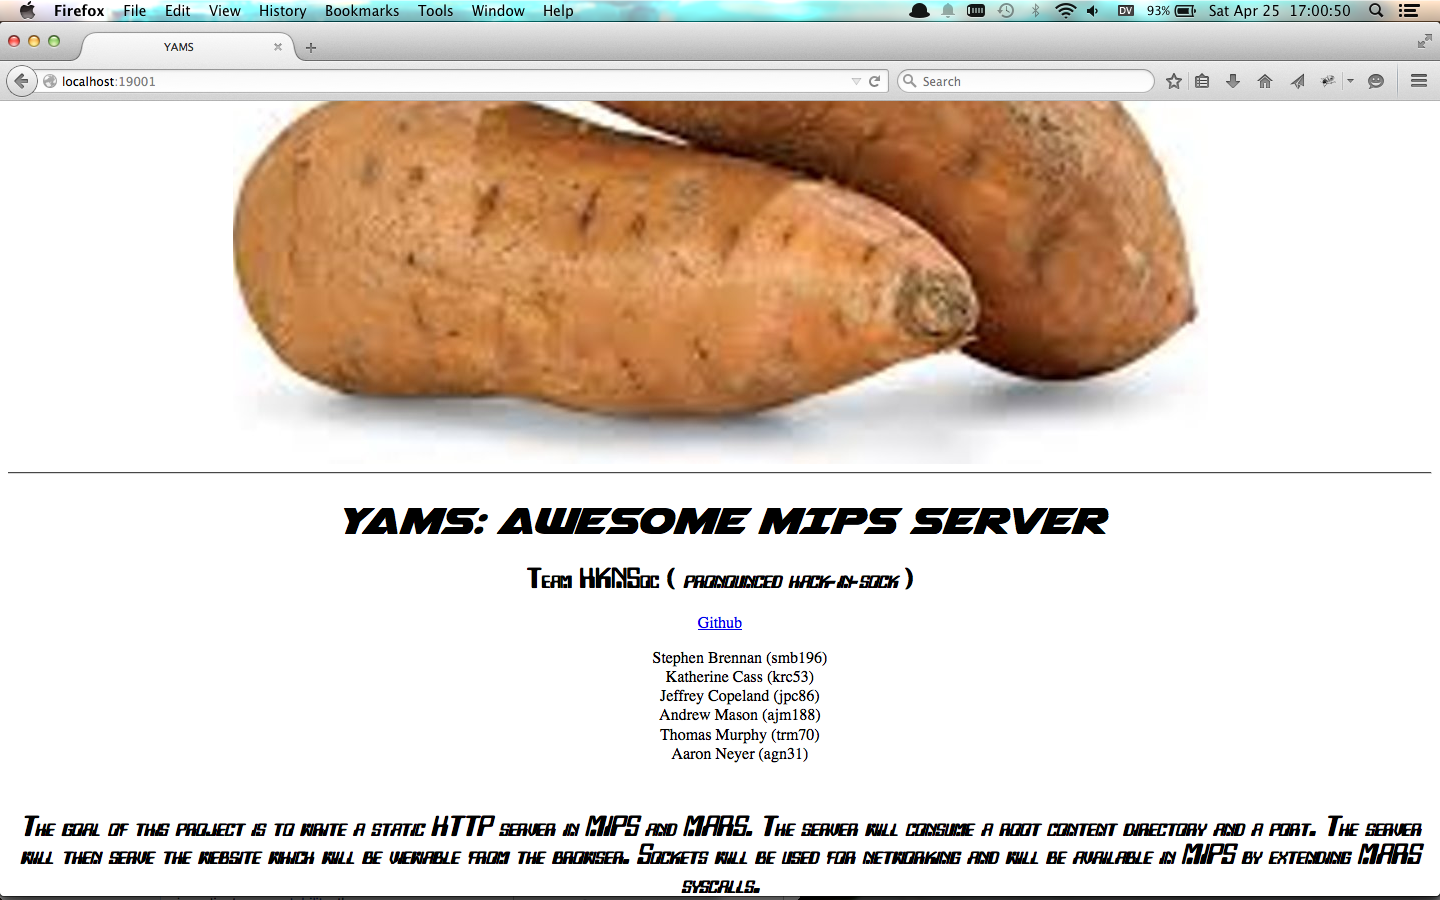
\includegraphics[width=0.8\textwidth,natwidth=1440,natheight=900]{static_document}
\caption{The static \texttt{index.html} served by YAMS by default.}
\label{fig:static_document}
\end{figure}

\begin{figure}[H]
\centering
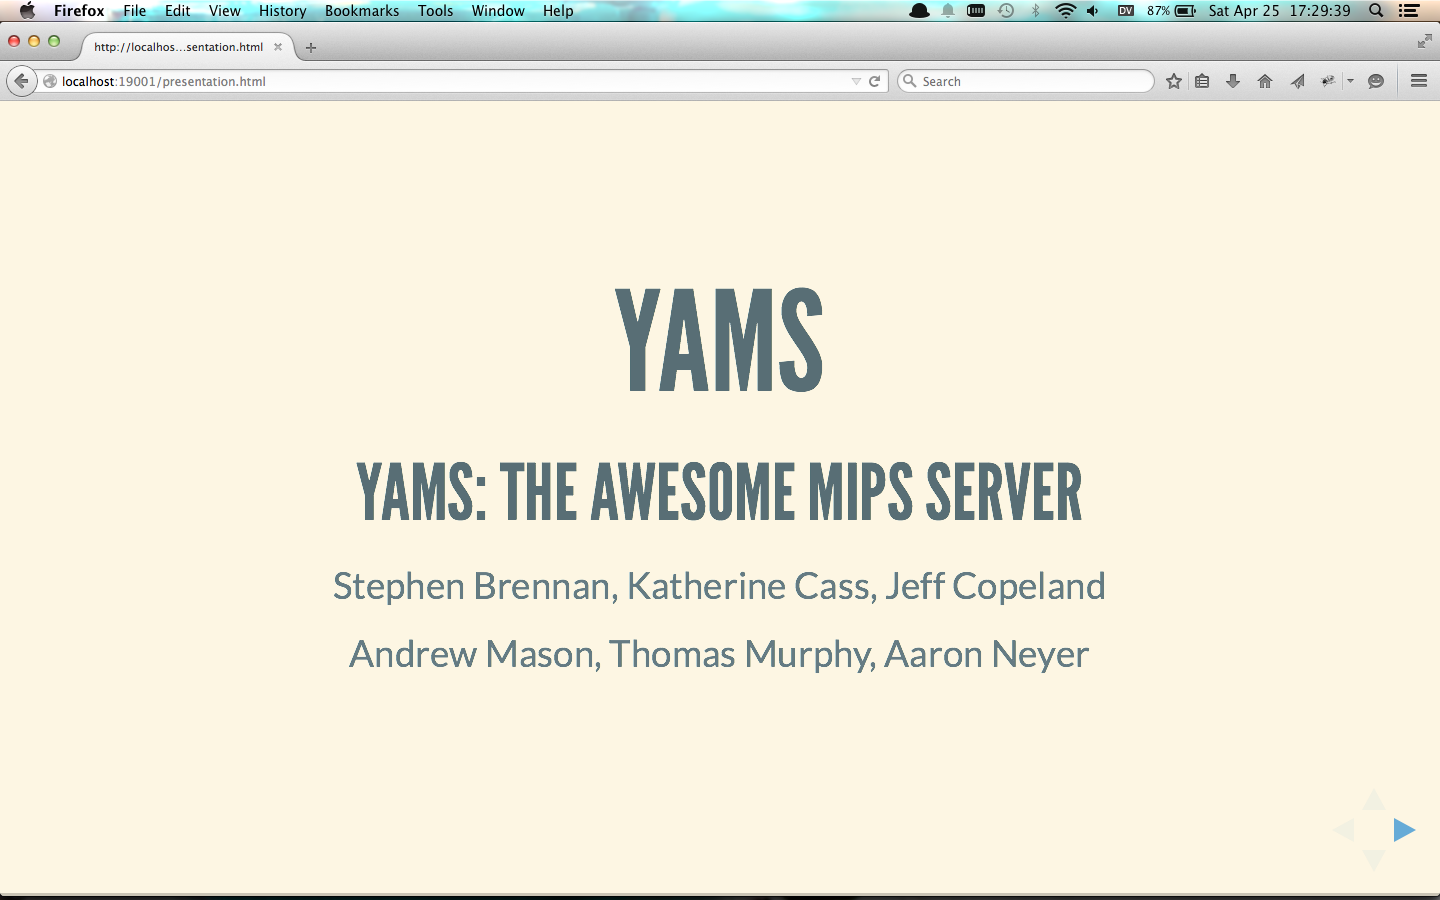
\includegraphics[width=0.8\textwidth,natwidth=1440,natheight=900]{dynamic_document}
\caption{The first view of a dynamic HTML/JavaScript page containing the material presented to the class.}
\label{fig:dynamic_document}
\end{figure}

\begin{figure}[H]
\centering
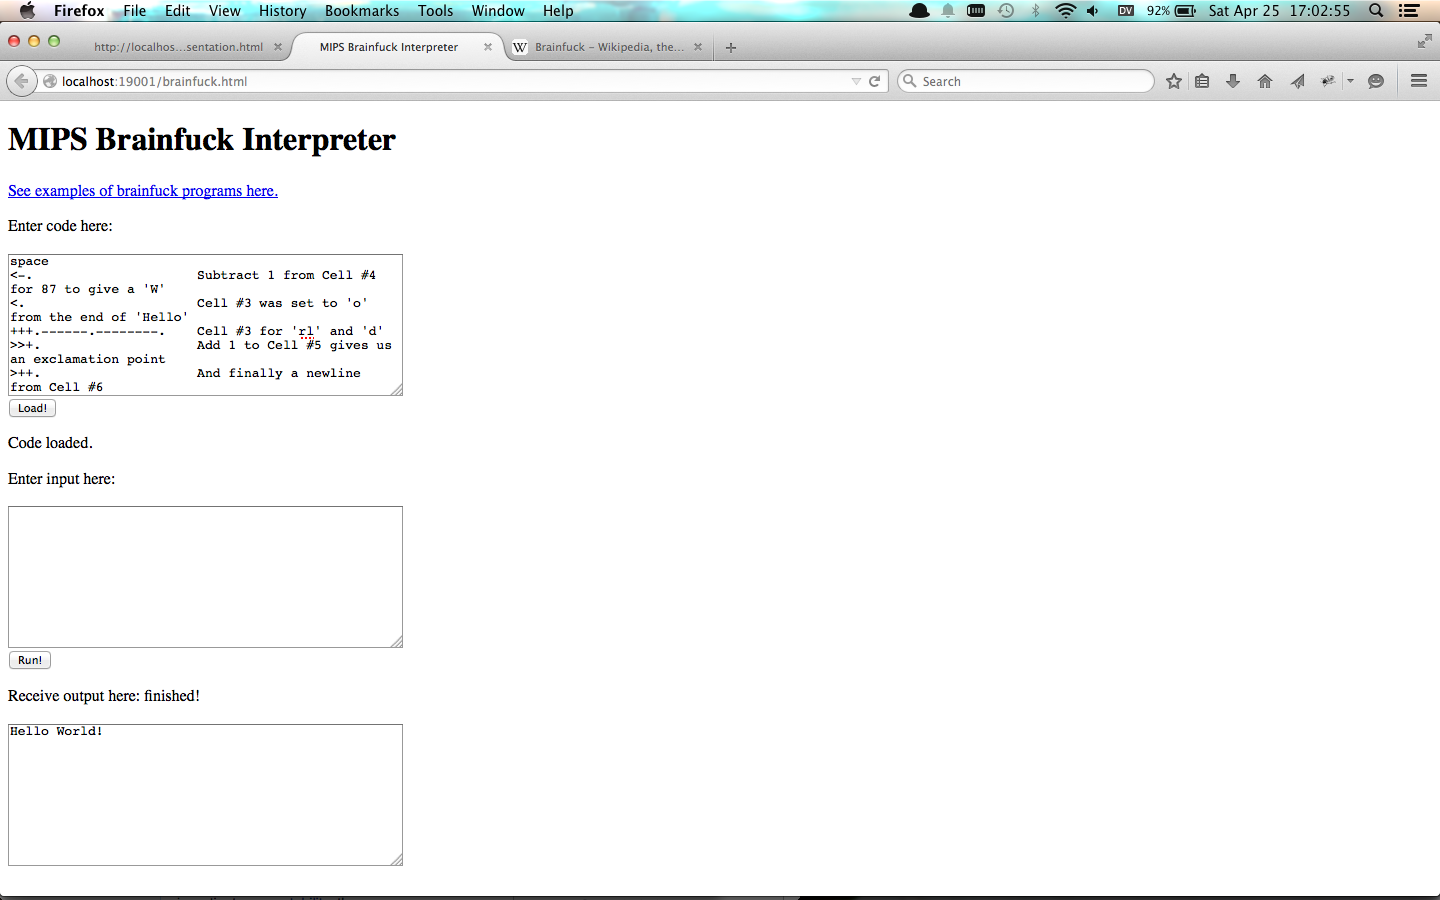
\includegraphics[width=0.8\textwidth,natwidth=1440,natheight=900]{interactive_ajax}
\caption{A web interface to an implementation of the Brainfuck interpreter contained within YAMS.}
\label{fig:interactive_ajax}
\end{figure}

\twocolumn

% use section* for acknowledgment
\section*{Acknowledgment}


The authors would like to thank Cameron Gutman
\texttt{\url{https://github.com/cgutman}} for providing information about the
usage of identity transfer encoding.


% Can use something like this to put references on a page
% by themselves when using endfloat and the captionsoff option.
\ifCLASSOPTIONcaptionsoff
  \newpage
\fi

% trigger a \newpage just before the given reference
% number - used to balance the columns on the last page
% adjust value as needed - may need to be readjusted if
% the document is modified later
%\IEEEtriggeratref{8}
% The "triggered" command can be changed if desired:
%\IEEEtriggercmd{\enlargethispage{-5in}}

% references section
\bibliography{IEEEabrv,./yams_report}
\bibliographystyle{IEEEtran}
\nocite{*}



% that's all folks
\end{document}
